\documentclass[a4paper,12pt]{article}

\usepackage{amsmath,amssymb,amsthm,multicol,tikz,enumitem}
\usepackage{hyperref}
\usepackage{fancyvrb}
%\usepackage{enumerate}
\usepackage[margin=2cm]{geometry}
\usetikzlibrary{calc,arrows.meta}

\newcommand\N{\mathbf{N}}
\newcommand\Q{\mathbf{Q}}
\newcommand\R{\mathbf{R}}
\newcommand\Z{\mathbf{Z}}

\def\ojoin{\setbox0=\hbox{$\bowtie$}%
  \rule[-.02ex]{.25em}{.4pt}\llap{\rule[\ht0]{.25em}{.4pt}}}
\def\leftouterjoin{\mathbin{\ojoin\mkern-5.8mu\bowtie}}
\def\rightouterjoin{\mathbin{\bowtie\mkern-5.8mu\ojoin}}
\def\fullouterjoin{\mathbin{\ojoin\mkern-5.8mu\bowtie\mkern-5.8mu\ojoin}}

% Comment out one or the other

\ifdefined\mysolution
  \newcommand\answer[1]{\mbox{}\\[-15pt]{\color{blue}{#1}}\hfill{\color{blue}$\qed$}\mbox{}\\[-15pt]} 
  \newcommand\ans[1]{{\color{blue}{#1}}}
\else 
  \newcommand\answer[1]{}
  \newcommand\ans[1]{}
\fi


\setlength{\parindent}{0pt}

\begin{document}

\thispagestyle{empty}

\begin{center}
{\bf\Huge Vidus eksāmens} \\[5pt]
Lietišķie algoritmi, 2019.g.\ rudens\\
Termiņš: 2019-10-29
\end{center}

\hrule
\vspace{2pt}
\hrule
\vspace{12pt}





\noindent
{\bf 1.uzdevums (1+1+1+2 punkti):}
Spēlētājs $X$ vienā gājienā izņem no urnas trīs kartiņas. 
Pieņemsim, ka urna ir ļoti liela, kartiņas tajā nekad nebeidzas un ir vienādas varbūtības
izķeksēt jebkuru no burtiem {\tt A}, {\tt B} vai {\tt C}; citu burtu urnā nav.
Pēc tam $X$ sakārto trīs kartiņas alfabētiskā secībā un nosūta spēlētājam $Y$ ziņojumu \textendash{} to burtu, kurš 
pēc sakārtošanas bija pirmais. (Piemēram, ja izķeksētie burti ir {\tt "CBC"}, tad pēc sakārtošanas tie būs {\tt "BCC"} un 
$X$ nosūta ziņojumu {\tt "B"}.) 
\begin{enumerate}
\item Kāds ir informācijas saturs ziņojumam {\tt A}?
\item Kāds ir informācijas saturs ziņojumam {\tt B}? 
\item Kāds ir informācijas saturs ziņojumam {\tt C}? 
\item Kāda ir entropija jebkuram vienam ziņojumam, ko $X$ nosūta $Y$ saskaņā ar augšminēto procedūru?
\end{enumerate}




\answer{


\begin{enumerate}
\item No visiem $27$ variantiem, kā izvilkt kartiņas, ir $9$ tādi, kas sākas ar burtu $\mathtt{A}$. Starp atlikušajiem
$18$ trešajai daļai (jeb $6$ variantiem) $\mathtt{A}$ ir otrajā pozīcijā. Visbeidzot, starp
atlikušajiem $27 - 9 - 6 = 12$ ir trešdaļa jeb $4$ tādi, kam $\mathtt{A}$ ir trešajā pozīcijā. Tātad
ziņojuma $\mathtt{A}$ varbūtība ir $(9+6+4)/(27) = 19/27$.\\
Informācijas saturs: $-\log_2\left(P(\mathtt{A})\right) \approx 0.507$.
\item Ziņojuma $\mathtt{B}$ varbūtība ir $7/27$ (no $1$ atņem ziņojumu $\mathtt{A}$ un $\mathtt{C}$ varbūtības).\\
Informācijas saturs ir $-\log_2\left(P(\mathtt{B})\right) \approx 1.948$.
\item Ziņojums {\tt C} var rasties vienīgi izvelkot kartiņas {\tt CCC}, tā varbūtība ir $p(\mathtt{C}) = 1/27$.\\
Informācijas saturs ir $-\log_2\left(P(\mathtt{C})\right) \approx 4.754$.
\item Entropija ir
$$-P(\mathtt{A})\log_2(P(\mathtt{A})) -P(\mathtt{B})\log_2(P(\mathtt{B})) - P(\mathtt{C})\log_2(P(\mathtt{C})) =$$
$$ = (19/27)\cdot 0.507 + (7/27)\cdot 1.948 + (1/27) \cdot 4.755 \approx 1.038.$$
\end{enumerate}


%pp <- c(19/27,7/27,1/27)
% round(log2(pp),digits=3)
%[1] -0.507 -1.948 -4.755



{\em Piezīme.} Variantu skaitu, kuros ir vismaz viens burts {\tt A} var saskaitīt arī citādi.
Ar $U$ apzīmējam visus tos variantus, kuros
pirmais burts ir {\tt "A"}, ar $V$ \textendash{} tos, kuros otrais burts ir {\tt "A"}, un ar
$W$ \textendash{} tos, kuros trešais burts ir {\tt "A"}; sk.\ Attēlu~\ref{fig:venn-diagram}. Viegli redzēt, ka elementu skaits
kopās $|U|=|V|=|W|=9$, elementu skaits kopu šķēlumos ir $|U \cap V| = |U \cap W| = |V \cap W| = 3$
(ir $3$ tādi varianti, kuros pirmais {\bf un} otrais burts ir {\tt "A"}). Savukārt visu
trīs kopu šķēlums $|U \cap V \cap W| = 1$ (atbilst gadījumam, kad visi trīs
burti ir {\tt "A"}).


\begin{figure}[htb!]
\begin{center}
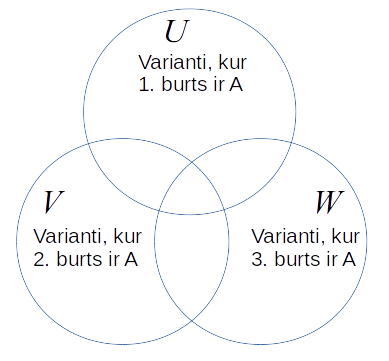
\includegraphics[width=0.3\textwidth]{fall2019-midterm/venn-diagram.png}
\caption{Kopu apvienojuma izteikšana ar ieslēgšanas-izslēgšanas principu\label{fig:venn-diagram}}
\end{center}
\end{figure}



Sk. \url{https://bit.ly/375cX4L} (ieslēgšanas-izslēgšanas principu),
kas ļauj noteikt elementu skaitu visu šo trīs kopu apvienojumā:
\[ \left| U \cup V \cup W \right| = \left| U \right| + \left| V \right| + \left| W \right| -
\left| U \cap V \right| - \left| U \cap W \right| - \left| V \cap W \right| + \left| U \cap V \cap W \right|. \]
\[ \left| U \cup V \cup W \right| = 9+9+9 - 3 - 3 - 3+1 = 19. \]
Citiem vārdiem, lai atrastu, cik elementu pieder kaut vienai no kopām $U,V,W$, saskaitām
šajās kopās esošos elementus ($|U|$, $|V|$ un $|W|$), tad atņemam tos, kurus esam pieskaitījuši
divreiz (kuri pieder kādam no divu kopu šķēlumiem
$|U \cap V|$, $|U \cap W|$ un $|V \cap W|$), visbeidzot pieskaitām atpakaļ
tos, kuri pieder visām trim ($|U \cap V \cap W$).

}




\vspace{6pt}
\noindent
{\bf 2.uzdevums (3 punkti - jebkāds pareizs Hafmana koks, 3 punkti - koks kanoniskajā formā):}
Hafmana koku sauksim par {\em kanonisku}, ja izpildās sekojošas īpašības: 
\begin{itemize}
\item Visi kanoniskā koka zari (ceļi no saknes līdz lapām/ziņojumiem) veido garumus, kuri ir nedilstošā secībā, skaitot no augšas uz leju.
\item Vienāda garuma zariem ziņojumi izkārtoti ziņojumu alfabētiskā secībā. 
\end{itemize}
Attēla 1.piemērā zaru garumi nav nedilstošā secībā
(zars $\mathtt{11}$ uz lapu $\mathtt{A}$ ir garumā $2$, virs tā divi zari garumā $3$). 
2.piemērā $\mathtt{C}$, $\mathtt{D}$ ir ar vienādi gariem kodavārdiem, bet nav alfabētiskā secībā.\\
Vienīgi 3.piemērā Hafmana koks ir kanonisks.

\begin{center}
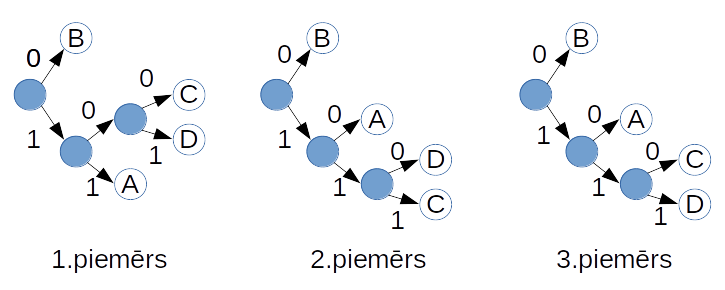
\includegraphics[width=0.5\textwidth]{fall2019-midterm/huffman-examples.png}
\end{center}

$5$ ziņojumu kopai $\{ \mathtt{A},\mathtt{B},\mathtt{C},\mathtt{D},\mathtt{E} \}$, kuru varbūtības ir attiecīgi 
${\displaystyle \left\{ \frac{1}{15}, \frac{2}{15},\frac{3}{15},\frac{4}{15},\frac{5}{15} \right\}}$,
atrast un uzzīmēt kanonisku Hafmana koku.


\answer{

Vispirms veidojam jebkādu Hafmana koku (kaut vai nekanonisku).
Sākumā mums ir $5$ mini-koki, šos kokus pierakstām kā pārīšus, piemēram,
$(\mathtt{A},1/15)$, kur ziņojums sapārots ar savu svaru.
Katrā nākamajā solī apvienojam divus vieglākos kokus lielākā kokā (koku, ko veido
apakškoki $t_1$ un $t_2$ apzīmējam ar $T(t_1,t_2)$) un saskaitām to svarus.

\begin{eqnarray}
 & & \left\{ \left( \mathtt{A}, \frac{1}{15} \right), \left( \mathtt{B}, \frac{2}{15} \right), \left( \mathtt{C}, \frac{3}{15} \right),
\left( \mathtt{D}, \frac{4}{15} \right), \left( \mathtt{E}, \frac{5}{15} \right) \right\} \\
 & \rightarrow & \left\{ \left( T(\mathtt{A},\mathtt{B}), \frac{3}{15} \right), \left( \mathtt{C}, \frac{3}{15} \right),
\left( \mathtt{D}, \frac{4}{15} \right), \left( \mathtt{E}, \frac{5}{15} \right) \right\} \\
 & \rightarrow & \left\{ \left( \mathtt{D}, \frac{4}{15} \right), \left( \mathtt{E}, \frac{5}{15} \right),
\left( T(T(\mathtt{A},\mathtt{B}), \mathtt{C}), \frac{6}{15} \right) \right\} \\
 & \rightarrow & \left\{ \left( T(T(\mathtt{A},\mathtt{B}), \mathtt{C}), \frac{6}{15} \right), \left( T(\mathtt{D},\mathtt{E}), \frac{9}{15} \right) \right\} \\
 & \rightarrow & \left\{ \left( T( T(T(\mathtt{A},\mathtt{B}), \mathtt{C}), T(\mathtt{D},\mathtt{E})), 1 \right) \right\}.
\end{eqnarray}

Uzzīmēsim (nekanonisko) Hafmana koku un pārveidosim to par kanonisku, sakārtojot zarus pēc garuma, un vienāda garuma zariem sarakstot
ziņojuma burtus alfabētiskā secībā, bet neizmainot ziņojumiem piešķirto Hafmana kodavārda garumus (sk.\ Attēlu~\ref{fig:huffman-canonical}). 
Tādējādi jaunizveidotais, kanoniskais Hafmana koks
ir ekvivalents sākotnējam (saglabā koda garumus visiem ziņojumiem), bet tam ir paredzamāka
struktūra un šo koku var iekodēt ar mazāk bitiem.

\begin{figure}[htb!]
\begin{center}
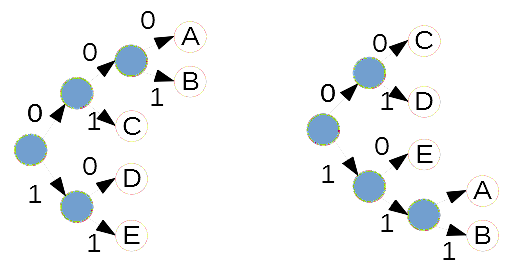
\includegraphics[width=0.4\textwidth]{fall2019-midterm/huffman-canonical.png}
\caption{Koka pārveidojums par kanonisku\label{fig:huffman-canonical}}
\end{center}
\end{figure}

}


\vspace{6pt}
{\bf 3.uzdevums (4 punkti):}
Izmantojot LZ78 algoritmu 6 simbolu alfabētam $\{\mathtt{C}, \mathtt{E}, \mathtt{L}, \mathtt{N},\mathtt{S}, \mathtt{U}\}$,
izveidot tabulu un nokodēt sekojošu $15$ simbolu ziņojumu: {\tt SUCCESSLESSNESS}. 
Tabulā attēlot soļa numuru, $w$ - garāko vārdnīcā jau atrodamo simbolu virkni, $k$ - virknei $w$ sekojošo simbolu, algoritma izvadi un 
vārdnīcai attiecīgajā solī pievienojamo vārdu. 

\begin{center}
\begin{tabular}{ |l|l|l|l|l| } \hline
Solis & $w$ & $k$ & Izvade & Pievieno vārdnīcai \\ \hline
$\ldots$ & $\ldots$ & $\ldots$ & $\ldots$ & $\ldots$ \\ \hline
\end{tabular}
\end{center}

\answer{


\begin{center}
\begin{tabular}{ |l|l|l|l|l| } \hline
Solis & $w$ & $k$ & Izvade & Pievieno vārdnīcai \\ \hline
1 & $\mathtt{S}$ & $\mathtt{U}$ & $\mathtt{S}$ & $\mathtt{SU}$ \\
2 & $\mathtt{U}$ & $\mathtt{C}$ & $\mathtt{U}$ & $\mathtt{UC}$ \\
3 & $\mathtt{C}$ & $\mathtt{C}$ & $\mathtt{C}$ & $\mathtt{CC}$ \\
4 & $\mathtt{C}$ & $\mathtt{E}$ & $\mathtt{C}$ & $\mathtt{CE}$ \\
5 & $\mathtt{E}$ & $\mathtt{S}$ & $\mathtt{E}$ & $\mathtt{ES}$ \\
6 & $\mathtt{S}$ & $\mathtt{S}$ & $\mathtt{S}$ & $\mathtt{SS}$ \\
7 & $\mathtt{S}$ & $\mathtt{L}$ & $\mathtt{S}$ & $\mathtt{SL}$ \\
8 & $\mathtt{L}$ & $\mathtt{E}$ & $\mathtt{L}$ & $\mathtt{LE}$ \\
9 & $\mathtt{ES}$ & $\mathtt{S}$ & $\mathtt{ES}\,\rightarrow\,5$ & $\mathtt{ESS}$ \\
10 & $\mathtt{S}$ & $\mathtt{N}$ & $\mathtt{S}$ & $\mathtt{SN}$ \\
11 & $\mathtt{N}$ & $\mathtt{E}$ & $\mathtt{N}$ & $\mathtt{NE}$ \\
12 & $\mathtt{ESS} $ & $\mathtt{[EOF]}$ & $\mathtt{ESS}\,\rightarrow\,9$ & $-$ \\ \hline
\end{tabular}
\end{center}

Nokodētais ziņojums ir $\mathtt{S.U.C.C.E.S.S.L.5.S.N.9}$.

}





\vspace{6pt}
{\bf 4.uzdevums (6 punkti):}
Veikt inverso Berouza-Vīlera transformāciju $17$ simbolu virknītei: {\tt SETTNRSDDIESIEESN}, 
ja zināms, ka kodētais vārds ir pats pirmais starp leksikogrāfiski sakārtotajām cikliskajām permutācijām. 

\answer{

Berouza-Vīlera atkodēšanu veicam vairākos soļos: Vienā solī pierakstām priekšā matricai kolonnu, kas
sakrīt ar atkodējamo virkni (solis {\tt add}), pēc tam
sakārtojam rindiņas alfabētiski (solis {\tt sort}). Minēto soli atkārto tik daudz reižu, cik
simbolu ir jāatkodē.

{\footnotesize
\[
\mathop{\longrightarrow}^{\text{add}}
\left(
\begin{array}{c}
\mathtt{S} \\
\mathtt{E} \\
\mathtt{T} \\
\mathtt{T} \\
\mathtt{N} \\
\mathtt{R} \\
\mathtt{S} \\
\mathtt{D} \\
\mathtt{D} \\
\mathtt{I} \\
\mathtt{E} \\
\mathtt{S} \\
\mathtt{I} \\
\mathtt{E} \\
\mathtt{E} \\
\mathtt{S} \\
\mathtt{N}
\end{array} \right)
\mathop{\longrightarrow}^{\text{sort}}
\left(
\begin{array}{c}
\mathtt{D} \\
\mathtt{D} \\
\mathtt{E} \\
\mathtt{E} \\
\mathtt{E} \\
\mathtt{E} \\
\mathtt{I} \\
\mathtt{I} \\
\mathtt{N} \\
\mathtt{N} \\
\mathtt{R} \\
\mathtt{S} \\
\mathtt{S} \\
\mathtt{S} \\
\mathtt{S} \\
\mathtt{T} \\
\mathtt{T}
\end{array} \right)
\mathop{\longrightarrow}^{\text{add}}
\left(
\begin{array}{c}
\mathtt{SD} \\
\mathtt{ED} \\
\mathtt{TE} \\
\mathtt{TE} \\
\mathtt{NE} \\
\mathtt{RE} \\
\mathtt{SI} \\
\mathtt{DI} \\
\mathtt{DN} \\
\mathtt{IN} \\
\mathtt{ER} \\
\mathtt{SS} \\
\mathtt{IS} \\
\mathtt{ES} \\
\mathtt{ES} \\
\mathtt{ST} \\
\mathtt{NT}
\end{array} \right)
\mathop{\longrightarrow}^{\text{sort}}
\left(
\begin{array}{c}
\mathtt{DI} \\
\mathtt{DN} \\
\mathtt{ED} \\
\mathtt{ER} \\
\mathtt{ES} \\
\mathtt{ES} \\
\mathtt{IN} \\
\mathtt{IS} \\
\mathtt{NE} \\
\mathtt{NT} \\
\mathtt{RE} \\
\mathtt{SD} \\
\mathtt{SI} \\
\mathtt{SS} \\
\mathtt{ST} \\
\mathtt{TE} \\
\mathtt{TE}
\end{array} \right)
\mathop{\longrightarrow}^{\text{add}}
\left(
\begin{array}{c}
\mathtt{SDI} \\
\mathtt{EDN} \\
\mathtt{TED} \\
\mathtt{TER} \\
\mathtt{NES} \\
\mathtt{RES} \\
\mathtt{SIN} \\
\mathtt{DIS} \\
\mathtt{DNE} \\
\mathtt{INT} \\
\mathtt{ERE} \\
\mathtt{SSD} \\
\mathtt{ISI} \\
\mathtt{ESS} \\
\mathtt{EST} \\
\mathtt{STE} \\
\mathtt{NTE}
\end{array} \right)
\mathop{\longrightarrow}^{\text{sort}}
\left(
\begin{array}{c}
\mathtt{DIS} \\
\mathtt{DNE} \\
\mathtt{EDN} \\
\mathtt{ERE} \\
\mathtt{ESS} \\
\mathtt{EST} \\
\mathtt{INT} \\
\mathtt{ISI} \\
\mathtt{NES} \\
\mathtt{NTE} \\
\mathtt{RES} \\
\mathtt{SDI} \\
\mathtt{SIN} \\
\mathtt{SSD} \\
\mathtt{STE} \\
\mathtt{TED} \\
\mathtt{TER} \\
\end{array} \right)
\mathop{\longrightarrow}^{\text{add}}
\left(
\begin{array}{c}
\mathtt{SDIS} \\
\mathtt{EDNE} \\
\mathtt{TEDN} \\
\mathtt{TERE} \\
\mathtt{NESS} \\
\mathtt{REST} \\
\mathtt{SINT} \\
\mathtt{DISI} \\
\mathtt{DNES} \\
\mathtt{INTE} \\
\mathtt{ERES} \\
\mathtt{SSDI} \\
\mathtt{ISIN} \\
\mathtt{ESSD} \\
\mathtt{ESTE} \\
\mathtt{STED} \\
\mathtt{NTER}
\end{array} \right)
\mathop{\longrightarrow}^{\text{sort}}
\left(
\begin{array}{c}
\mathtt{DISI} \\
\mathtt{DNES} \\
\mathtt{EDNE} \\
\mathtt{ERES} \\
\mathtt{ESSD} \\
\mathtt{ESTE} \\
\mathtt{INTE} \\
\mathtt{ISIN} \\
\mathtt{NESS} \\
\mathtt{NTER} \\
\mathtt{REST} \\
\mathtt{SDIS} \\
\mathtt{SINT} \\
\mathtt{SSDI} \\
\mathtt{STED} \\
\mathtt{TEDN} \\
\mathtt{TERE}
\end{array} \right)
\]

\[
\mathop{\longrightarrow}^{\text{add}}
\left(
\begin{array}{c}
\mathtt{SDISI} \\
\mathtt{EDNES} \\
\mathtt{TEDNE} \\
\mathtt{TERES} \\
\mathtt{NESSD} \\
\mathtt{RESTE} \\
\mathtt{SINTE} \\
\mathtt{DISIN} \\
\mathtt{DNESS} \\
\mathtt{INTER} \\
\mathtt{EREST} \\
\mathtt{SSDIS} \\
\mathtt{ISINT} \\
\mathtt{ESSDI} \\
\mathtt{ESTED} \\
\mathtt{STEDN} \\
\mathtt{NTERE}
\end{array} \right)
\mathop{\longrightarrow}^{\text{sort}}
\left(
\begin{array}{c}
\mathtt{DISIN} \\
\mathtt{DNESS} \\
\mathtt{EDNES} \\
\mathtt{EREST} \\
\mathtt{ESSDI} \\
\mathtt{ESTED} \\
\mathtt{INTER} \\
\mathtt{ISINT} \\
\mathtt{NESSD} \\
\mathtt{NTERE} \\
\mathtt{RESTE} \\
\mathtt{SDISI} \\
\mathtt{SINTE} \\
\mathtt{SSDIS} \\
\mathtt{STEDN} \\
\mathtt{TEDNE} \\
\mathtt{TERES}
\end{array} \right)
\mathop{\longrightarrow}^{\text{add}}
\left(
\begin{array}{c}
\mathtt{SDISIN} \\
\mathtt{EDNESS} \\
\mathtt{TEDNES} \\
\mathtt{TEREST} \\
\mathtt{NESSDI} \\
\mathtt{RESTED} \\
\mathtt{SINTER} \\
\mathtt{DISINT} \\
\mathtt{DNESSD} \\
\mathtt{INTERE} \\
\mathtt{ERESTE} \\
\mathtt{SSDISI} \\
\mathtt{ISINTE} \\
\mathtt{ESSDIS} \\
\mathtt{ESTEDN} \\
\mathtt{STEDNE} \\
\mathtt{NTERES}
\end{array} \right)
\mathop{\longrightarrow}^{\text{sort}}
\left(
\begin{array}{c}
\mathtt{DISINT} \\
\mathtt{DNESSD} \\
\mathtt{EDNESS} \\
\mathtt{ERESTE} \\
\mathtt{ESSDIS} \\
\mathtt{ESTEDN} \\
\mathtt{INTERE} \\
\mathtt{NESSDI} \\
\mathtt{NTERES} \\
\mathtt{ISINTE} \\
\mathtt{RESTED} \\
\mathtt{SDISIN} \\
\mathtt{SINTER} \\
\mathtt{SSDISI} \\
\mathtt{STEDNE} \\
\mathtt{TEDNES} \\
\mathtt{TEREST}
\end{array} \right)
\mathop{\longrightarrow}^{\text{add}}
\left(
\begin{array}{c}
\mathtt{SDISINT} \\
\mathtt{EDNESSD} \\
\mathtt{TEDNESS} \\
\mathtt{TERESTE} \\
\mathtt{NESSDIS} \\
\mathtt{RESTEDN} \\
\mathtt{SINTERE} \\
\mathtt{DISINTE} \\
\mathtt{DNESSDI} \\
\mathtt{INTERES} \\
\mathtt{ERESTED} \\
\mathtt{SSDISIN} \\
\mathtt{ISINTER} \\
\mathtt{ESSDISI} \\
\mathtt{ESTEDNE} \\
\mathtt{STEDNES} \\
\mathtt{NTEREST}
\end{array} \right)
\mathop{\longrightarrow}^{\text{sort}}
\left(
\begin{array}{c}
\mathtt{DISINTE} \\
\mathtt{DNESSDI} \\
\mathtt{EDNESSD} \\
\mathtt{ERESTED} \\
\mathtt{ESSDISI} \\
\mathtt{ESTEDNE} \\
\mathtt{INTERES} \\
\mathtt{ISINTER} \\
\mathtt{NESSDIS} \\
\mathtt{NTEREST} \\
\mathtt{RESTEDN} \\
\mathtt{SDISINT} \\
\mathtt{SINTERE} \\
\mathtt{SSDISIN} \\
\mathtt{STEDNES} \\
\mathtt{TEDNESS} \\
\mathtt{TERESTE}
\end{array} \right)
\]
\[
\mathop{\longrightarrow}^{\text{add}}
\left(
\begin{array}{c}
\mathtt{SDISINTE} \\
\mathtt{EDNESSDI} \\
\mathtt{TEDNESSD} \\
\mathtt{TERESTED} \\
\mathtt{NESSDISI} \\
\mathtt{RESTEDNE} \\
\mathtt{SINTERES} \\
\mathtt{DISINTER} \\
\mathtt{DNESSDIS} \\
\mathtt{INTEREST} \\
\mathtt{ERESTEDN} \\
\mathtt{SSDISINT} \\
\mathtt{ISINTERE} \\
\mathtt{ESSDISIN} \\
\mathtt{ESTEDNES} \\
\mathtt{STEDNESS} \\
\mathtt{NTERESTE}
\end{array} \right)
\mathop{\longrightarrow}^{\text{sort}}
\left(
\begin{array}{c}
\mathtt{DISINTER} \\
\mathtt{DNESSDIS} \\
\mathtt{EDNESSDI} \\
\mathtt{ERESTEDN} \\
\mathtt{ESSDISIN} \\
\mathtt{ESTEDNES} \\
\mathtt{INTEREST} \\
\mathtt{ISINTERE} \\
\mathtt{NESSDISI} \\
\mathtt{NTERESTE} \\
\mathtt{RESTEDNE} \\
\mathtt{SDISINTE} \\
\mathtt{SINTERES} \\
\mathtt{SSDISINT} \\
\mathtt{STEDNESS} \\
\mathtt{TEDNESSD} \\
\mathtt{TERESTED}
\end{array} \right)
\mathop{\longrightarrow}^{\text{add}}
\left(
\begin{array}{c}
\mathtt{SDISINTER} \\
\mathtt{EDNESSDIS} \\
\mathtt{TEDNESSDI} \\
\mathtt{TERESTEDN} \\
\mathtt{NESSDISIN} \\
\mathtt{RESTEDNES} \\
\mathtt{SINTEREST} \\
\mathtt{DISINTERE} \\
\mathtt{DNESSDISI} \\
\mathtt{INTERESTE} \\
\mathtt{ERESTEDNE} \\
\mathtt{SSDISINTE} \\
\mathtt{ISINTERES} \\
\mathtt{ESSDISINT} \\
\mathtt{ESTEDNESS} \\
\mathtt{STEDNESSD} \\
\mathtt{NTERESTED}
\end{array} \right)
\mathop{\longrightarrow}^{\text{sort}}
\left(
\begin{array}{c}
\textcolor{red}{\mathtt{DISINTERE}} \\
\mathtt{DNESSDISI} \\
\mathtt{EDNESSDIS} \\
\mathtt{ERESTEDNE} \\
\mathtt{ESSDISINT} \\
\textcolor{red}{\mathtt{ESTEDNESS}} \\
\mathtt{INTERESTE} \\
\mathtt{ISINTERES} \\
\mathtt{NESSDISIN} \\
\mathtt{NTERESTED} \\
\mathtt{RESTEDNES} \\
\mathtt{SDISINTER} \\
\mathtt{SINTEREST} \\
\mathtt{SSDISINTE} \\
\mathtt{STEDNESSD} \\
\mathtt{TEDNESSDI} \\
\mathtt{TERESTEDN}
\end{array} \right)
\]
}

Atkodēšanas procedūru varētu turpināt, bet ievērojam, ka šajā brīdī jau atkodēti $9$ simboli no $17$, turklāt
atkodējamais vārds ir leksikogrāfiski pirmais. Tādēļ arī, pierakstot atlikušos simbolus, tas sāksies ar
prefiksu {\tt DISINTERE}. Ievērojam arī, ka pirms burtiem {\tt DIS} cikliskajās permutācijās vienmēr parādās
burti {\tt SS}. Tātad atkodējamā virkne beidzas ar {\tt SS}. Vienīgā šāda virkne ir sestajā rindiņā.
Abas virknes sarakstot kopā, iegūstam meklēto vārdu:
\[ \lefteqn{\overbrace{\phantom{\mathtt{DISINTERE}}}}\mathtt{DISINTER}\!\underbrace{\mathtt{ESTEDNESS}} \]
Abas virknes ir garumā $9$, bet atkodējamais vārds ir $17$ zīmes garš, tādēļ vidējais burts "E" ir kopīgs abām
virknēm.

}


\vspace{6pt}
{\bf 5.uzdevums (2+3 punkti):} 
Kvantizācijas algoritms saņem ieejā attēla krāsu intensitātes, kuras ir veseli skaitļi 
$x \in \{ 0, 1,2,\ldots,255 \}$ un atgriež apakšējo veselo daļu: ${\displaystyle \left\lfloor \frac{x}{10} \right\rfloor}$
jeb nomet tā decimālpieraksta pēdējo ciparu. 
\begin{enumerate}
\item 
Ja visas šīs kvantizētās vērtības būtu jāsūta, izmantojot vienādu, fiksētu bitu skaitu \textendash{} cik lielu saspiešanas 
attiecību ({\em compression ratio} \textendash{} sākotnējā faila izmēra attiecību pret saspiestā faila izmēru) varētu sasniegt?
\item
Pieņemot, ka visas krāsu intensitātes (no $0$ līdz $255$) ir ar vienādām varbūtībām, 
kāda ir jaunās, kvantizētās ziņojumu virknes entropija? Kāda būtu teorētiski labākā iespējamā saspiešanas attiecība (ja izmantotu
aritmētisko kodējumu vai citu optimālu metodi, kas tuvojas entropijas noteiktajai saspiešanas robežai).
\end{enumerate}


\answer{

\begin{enumerate}
\item Pēc kvantizēšanas var rasties jebkurš no skaitļiem $0,1,2,\ldots,25$ \textendash{} pavisam $26$ vērtības.
Katras vērtības nokodēšanai pietiek ar $5$ bitiem, jo var izveidot $2^{5} = 32$ dažādus $5$-bitu kodus.
Katrai no $26$ vērtībām būs savs piecbitu kods (un vēl $6$ piecbitu kodi paliks neizmantoti).
Esam ieguvuši, ka ikvienu $8$-bitu vērtību (no $0$ līdz $255$) pēc kvantizācijas var iekodēt $5$ bitos.
Šī ir zudumradošā saspiešana un failu saspiešanas attiecība ({\em compression ratio}) sanāk $8/5 = 1.6$.\\
{\em Piezīme.} Praksē saspiešanas attiecība var sanākt nedaudz mazāka par $1.6$, jo neviens fails nevar
saturēt bitu skaitu, kas nedalās ar $8$ (t.i.\ neveselu skaitu baitu).
Tāpēc faila beigās daži biti ies zudumā (un, lai zinātu kur apstāties,
var nākties ieviest kodējuma beigu simbolu $\mathtt{[EOT]}$ kā $27$-to ziņojumu attēla beigās.)
\item Jebkurai kvantizācijas vērtībai no $0$ līdz $24$ ir vienāda varbūtība: $\frac{10}{256}$, bet
pašai pēdējai vērtībai ($25$) ir varbūtība $\frac{6}{256}$. Entropiju iegūstam, saskaitot
negatīvos logaritmus šīm varbūtībām, kas piereizināti ar pašām varbūtībām:
$$ \underbrace{-\frac{10}{256}\log_2\left( \frac{10}{256} \right) - \ldots - \frac{10}{256}\log_2\left( \frac{10}{256} \right)}_{25\,\text{saskaitāmie}} - \frac{6}{256}\log_2\left( \frac{6}{256} \right) = $$
$$ = -25\cdot \frac{10}{256}\log_2\left( \frac{10}{256} \right) - 1 \cdot \frac{6}{256}\log_2\left( \frac{6}{256} \right) \approx 4.695345.$$
Esam ieguvuši, ka taupīgāk kodējot šīs kvantificētās vērtības, tās var nosūtīt, tērējot vidēji $4.695345$ bitus vienai vērtībai,
nevis tieši $5$ bitus, kā sanāca iepriekšējā punktā.\\
Starp citu $\log_2(26) = 4.70044$, t.i.\ pat pieņemot, ka visām $26$ kvantificētajām vērtībām ir vienādas varbūtības (nevis pašai
pēdējai drusku mazāka varbūtība kā citām), kodējuma garums izmainās ļoti nedaudz.
\end{enumerate}


}


\vspace{6pt}
{\bf 6.uzdevums (4 punkti):}
Spēlētājs $X$ vēlas nosūtīt spēlētājam $Y$ dažus ceturtās pakāpes polinomus ar veseliem koeficientiem: 
$$f(x) = a_0x^4 + a_1x^3 + a_2x^2 + a_3x + a_4,\;\;\text{kur}\;\;a_0,\ldots,a_4 \in \mathbb{Z}.$$
Polinoma koeficientu $a_i$ vietā spēlētājs $X$ sūta $s$ vērtības dažādiem veseliem argumentiem: 
$$f(0),f(1),\ldots,f(s-1).$$
Vidū starp spēlētājiem $X$ un $Y$ atrodas ļaunprātīgais Šlopsterklopsters, kurš ne vairāk kā piecas
no visām $s$ nosūtītajām vērtībām drīkst nomainīt ar citiem skaitļiem (bet drīkst nomainīt arī mazāku skaitu 
vērtību vai nenomainīt nevienu).\\
Uzrakstīt nevienādību attiecībā pret parametru $s$ (un atrisināt to), lai uzzinātu mazāko polinoma vērtību skaitu $s$, kuram
spēlētājs $Y$ noteikti varēs atjaunot $X$'a sūtīto polinomu, lai kā arī nerīkotos Šlopsterklopsters.


\answer{

Ievērosim, ka diviem {\bf dažādiem} ceturtās pakāpes polinomiem
$f(x)$ un $g(x)$ var sakrist vērtības ne vairāk kā
četros punktos. (Šo polinomu starpība $f(x)-g(x)$ pati ir ne vairāk kā ceturtās pakāpes polinoms.
Un tāpēc šai starpībai $f(x) - g(x) = 0$ var būt ne vairāk kā $4$ dažādas saknes saskaņā ar
algebras pamatteorēmu; sk. \url{https://en.wikipedia.org/wiki/Fundamental_theorem_of_algebra}.

Ja polinoma vērtību pārsūtīšanā Šlopsterklopsters drīkst ieviest ne vairāk kā $c=5$ kļūdas,
tad katriem diviem polinomiem $f(x)$ un $g(x)$, kurus $X$ sūta spēlētājam $Y$, jānodrošina, lai vismaz $11$ no
pārsūtāmajām vērtībām (pirms to sabojāšanas) atšķirtos. Pretējā gadījumā, ja izrādītos, ka
atšķiras tikai $10$ vērtības, Šlopsterklopsters tieši pusi no pārsūtāmā polinoma $f(x)$ vērtībām aizstās ar $g(x)$ vērtībām 
(vai otrādi). Tad saņēmējs $Y$ šos polinomus nevarēs atšķirt.

Tā kā dažādiem polinomiem $f(x)$ un $g(x)$ vērtības pie četrām argumentu vērtībām drīkst sakrist 
arī bez jebkādas datu sabojāšanas (algebras pamatteorēma), bet vismaz $11$ vērtībām jābūt atšķirīgām, tad 
kopīgais pārsūtāmo vērtību skaits $s$ apmierina nevienādību: 
$$s - 4 \geq 11,\;\;\text{jeb}\;\;s \geq 15.$$
Lekciju konspektos šo nevienādību parasti pierakstījām šādi:
$$s - (k-1) \geq 2c + 1,$$
kur $s$ \textendash{} pārsūtāmo vērtību skaits; $k$ \textendash{} polinoma koeficientu skaits (un $k-1$ \textendash{} 
polinoma pakāpe), bet $c$ \textendash{} maksimāli atļautais kļūdu skaits.
Sk. \url{https://bit.ly/2MXyJxZ}. 

Ja pārsūta mazāk kā $15$ polinoma vērtības, tad var viegli izveidot pretpiemērus. Iedomāsimies, ka 
spēlētājs $X$ pārsūta vērtības tikai $14$ punktos: argumentiem $x \in \{ 0,1,\ldots,12,13 \}$. 
Definējam divus 4.pakāpes polinomus, katram no kuriem ir pieci koeficienti:
$$ \left\{ 
\begin{array}{l}
f(x) = (x-1)(x-5)(x-9)(x-13) = 1 x^4 - 28 x^3 + 254 x^2 - 812x + 585,\\
g(x) = 2(x-1)(x-5)(x-9)(x-13) = 2 x^4 - 56 x^3 + 508 x^2 - 1624x + 1170.
\end{array} \right.$$

Tās konstruētas tā, lai četras to vērtības sakristu, ja $x = 1,5,9,13$. Šlopsterklopsters 
pārsūta visas šīs četras sakrītošās vērtības, kā arī piecas $f(x)$ vērtības (zaļais grafiks Attēlā~\ref{fig:reed-solomon-plot}) un 
vēl piecas $g(x)$ vērtības (zilais grafiks Attēlā~\ref{fig:reed-solomon-plot}). Tā kā spēlētājs $Y$ nezina, kuras vērtības 
tiks sabojātas, viņš no saņemtajiem sarkanajiem punktiem nevar viennozīmīgi secināt, vai spēlētājs $X$ 
sūtīja polinomu $f(x)$ vai polinomu $g(x)$. 

Tas nozīmē, ka $f(x)$ un $g(x)$ attiecīgo koeficientu pārraidīšanai ar Rīda-Solomona kļūdu korekcijas algoritmu, 
kur atļautas piecas kļūdas, jānosūta vismaz $s = 15$ vērtības. 

\begin{figure}[h!]
\begin{center}
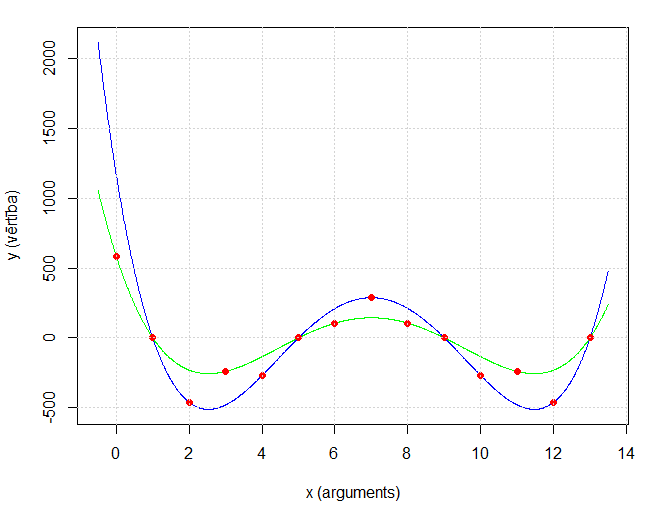
\includegraphics[width=0.7\textwidth]{fall2019-midterm/reed-solomon-plot.png}
\caption{Sarkanie punkti neļauj atšķirt $f(x)$ un $g(x)$\label{fig:reed-solomon-plot}}
\end{center}
\end{figure}

}



\vspace{6pt}
{\bf 7.uzdevums (2+2+2 punkti):} 
(Ieteikums: Šajā uzdevumā var izmantot algebriskas identitātes par skaitļu kāpināšanu, Eilera teorēmu u.c. skaitļu teorijas rezultātus.)
\begin{enumerate}
\item Kriptogrāfijas algoritmam ir jāaprēķina $4^{143}\;(\text{mod}\,199)$ (atlikums, kas rodas dalot $4^{139}$ ar $199$). 
Algoritms var ielūkoties reizināšanas tabulā pēc moduļa $199$: ievadīt divus skaitļus $a,b$ un saņemt to reizinājumu 
$a\cdot{}b\;(\text{mod}\,199)$ ($ab$ atlikumu, dalot ar $199$).
Kādu mazāko reižu skaitu pietiek ielūkoties reizināšanas tabulā, lai atrastu $4^{139}\;(\text{mod}\,199)$.\\
{\em Piezīme.} Algoritms var veikt arī dalīšanu ar atlikumu un atņemšanu, bet jāsaskaita tikai reizināšanas darbības.
(Acīmredzot, pietiek veikt $142$ reizināšanas; Jūsu uzdevums ir reizināšanu skaitu pēc iespējas samazināt.)
\item Kriptogrāfijas algoritmam ir jāaprēķina $4^{143}\;(\text{mod}\,7)$. Algoritms var ielūkoties reizināšanas tabulā 
pēc moduļa $7$. Kādu mazāko reizināšanu skaitu vajag, lai atrastu rezultātu? 
\item Atrast $4^{143}\;(\text{mod}\,7)$ vērtību; parādīt, kā tā iegūta.
\end{enumerate}

\answer{

\begin{enumerate}
\item Izsakām $143$ binārajā pierakstā: $143_{10} = 128 + 8 + 4 + 2 + 1 = 10001111_2$.
Lai uzzinātu, cik ir $4^{143}$, sareizināsim $4^{128}4^{8}4^{4}4^{2}4^1$ (tās ir $4$ reizināšanas). \\
Lai noskaidrotu skaitļus $4^2, 4^4, 4^8, 4^{16}, 4^{32}, 4^{64}, 4^{128}$, nepieciešamas vēl $7$ reizināšanas
(katru skaitli šajā virknē noskaidro, kāpinot iepriekšējo skaitli kvadrātā). Tātad, lai kāpinātu skaitļus $143$ pakāpē,
nepieciešamas pavisam $4+7 = 11$ reizināšanas darbības.
\item Lai uzzinātu $4^{143}\;(\text{mod}\,7)$, vispirms pielietosim Eilera teorēmu.
Šajā gadījumā kāpinātājs $143$ ir daudz lielāks par moduli, kas ir $7$, tāpēc augstām pakāpēm
vērtības pēc moduļa $7$ būs ieciklējušās (un cikls ir $\varphi(7) = 6$).\\
Tāpēc šoreiz vislabāk ir vispirms izdalīt $143$ ar $6$ (iegūstot atlikumu $5$).
Lai kāpinātu skaitli 5.pakāpē, nepieciešamas četras reizināšanas darbības.
\item Pēc Eilera teorēmas, katram skaitlim $a$, kas nedalās ar $7$, ir spēkā $a^{6} \equiv 1\;(\text{mod}\,7)$.
Tai skaitā $4^6 \equiv 1\;(\text{mod}\,7)$:
\[ 4^{138+5} = 4^{6\cdot{}23+5} = (4^6)^{23} \cdot{} 4^5 \equiv 1^{23} \cdot{} 4^5 = 4^3 \cdot 4^2 = 64 \cdot 16. \]
$64$ atlikums, dalot ar $7$ ir $1$, bet $16$ atlikums, dalot ar $7$ ir $2$. To reizinājums ir $1 \cdot 2 = 2$.
\end{enumerate}

}


\end{document}



